% 第5章第5节：赋范空间（范数与收敛、有限维赋范空间、完备性与Banach空间），只讨论有限维情形。

\section{赋范空间}
\label{sec:ls-normed-spaces}

上一章只用到加法与数乘，回答的都是“能否表示、是否唯一、有几个方向”这类是非与计数问题，还没有“大小”。可是用一个多项式近似一个函数时，要问误差有多大；一列近似越来越好时，要问它们是否趋于某个对象，那个对象是否仍在原来的空间里；上一章的读取也要问，输入不大时读数最多有多大。第~\ref{chap:linear-operations}章用范数度量$\mathbb R^d$中数组的大小，本节把它推广到一般线性空间。

本节回答三个问题：范数怎样给出收敛；有限维空间中，选哪个范数会不会影响收敛与否；收敛序列的极限什么时候一定留在空间中。前两个问题在有限维中有干净的答案：一切范数等价，收敛就是逐坐标收敛。第三个问题引出完备性与Banach空间，它在有限维中自动成立。本节只讨论有限维空间；无限维空间仍可用范数定义收敛，但范数等价与完备性不再自动成立，留到后面的章节。

\subsection{范数、距离与收敛}
\label{sec:ls-normed-space-definition}

\paragraph{范数的定义}
第~\ref{chap:linear-operations}章的$\ell_1$、$\ell_2$、$\ell_\infty$范数各有侧重，所表达的大小应满足同样的几条要求：大小非负，只有零向量大小为零，整体放大$c$倍时大小放大$|c|$倍，两段误差相加时总大小不超过各自大小之和。这些要求只用到加法与数乘，因此可以直接作为一般线性空间上“大小”的要求。
\begin{definition}[赋范空间]
\label{def:ls-normed-space}
\label{def:functional-normed-space}
设$V$是实线性空间。映射$\lVert\cdot\rVert:V\to[0,\infty)$若对任意$\bm x,\bm y\in V$与$c\in\mathbb R$满足
\begin{enumerate}
 \item 正定性：$\lVert\bm x\rVert=0$当且仅当$\bm x=\bm0$；
 \item 齐次性：$\lVert c\bm x\rVert=|c|\,\lVert\bm x\rVert$；
 \item 三角不等式：$\lVert\bm x+\bm y\rVert\leq\lVert\bm x\rVert+\lVert\bm y\rVert$，
\end{enumerate}
就称为$V$上的\term{范数}（norm）；配备范数的线性空间$(V,\lVert\cdot\rVert)$称为\term{赋范空间}（normed space）。
\end{definition}
范数诱导距离$d(\bm x,\bm y)=\lVert\bm x-\bm y\rVert$：它非负，只在$\bm x=\bm y$时为零，对称，并满足$d(\bm x,\bm z)\leq d(\bm x,\bm y)+d(\bm y,\bm z)$。这些性质也是\BookChapterRef{chap:metric-spaces}{第~\ref{chap:metric-spaces}章}度量空间的公理，所以赋范空间是一类特殊的度量空间。它的距离还与线性运算相容：平移不改变距离，缩放把距离按比例缩放。

把三角不等式用于$\bm x=(\bm x-\bm y)+\bm y$，得$\lVert\bm x\rVert-\lVert\bm y\rVert\leq\lVert\bm x-\bm y\rVert$；交换$\bm x,\bm y$的角色，又得$\lVert\bm y\rVert-\lVert\bm x\rVert\leq\lVert\bm x-\bm y\rVert$。两式合起来就是反向三角不等式
\begin{equation}
 \bigl|\lVert\bm x\rVert-\lVert\bm y\rVert\bigr|\leq\lVert\bm x-\bm y\rVert,
 \label{eq:ls-reverse-triangle}
\end{equation}
它说明两个向量相距很近时，长度也相差很少。

\paragraph{坐标范数的公理检验}
\label{sec:ls-norms-distances}
\label{sec:linear-algebra-distance-relations}

第~\ref{sec:ls-vector-operations}节的$p$范数满足非负性、正定性与齐次性，这可以直接从公式读出；需要证明的是三角不等式。$p=1$时，对每个坐标用实数的$|x_j+y_j|\leq|x_j|+|y_j|$再求和即得；$p=\infty$时，同一不等式给出$|x_j+y_j|\leq\lVert\bm x\rVert_\infty+\lVert\bm y\rVert_\infty$，再对$j$取最大值即得。$1<p<\infty$时，先要建立下面的不等式，它用一对互相配合的$p$范数与$q$范数控制两个向量逐项乘积之和。

\paragraph{Hölder不等式}
先估计两个向量逐坐标相乘后的总和。下面的共轭指数条件使两个范数能够配合使用。
\begin{theorem}[有限维Hölder不等式]
\label{thm:linear-algebra-holder}
设$1\leq p,q\leq\infty$且$1/p+1/q=1$（约定$1/\infty=0$），则$|\bm x^\top\bm y|\leq\lVert\bm x\rVert_p\lVert\bm y\rVert_q$。
\end{theorem}
\begin{proof}
先设$1<p,q<\infty$，分三步证明。

第一步，证明Young不等式：对$u,v\geq0$，
\[
 uv\leq\frac{u^p}{p}+\frac{v^q}{q}.
\]
$u=0$时左侧为零，不等式成立。$u>0$时令$t=v/u^{p-1}\geq0$。由$1/p+1/q=1$得$(p-1)q=p$，于是$v^q=t^qu^p$、$uv=tu^p$，不等式化为
\[
 u^p\Bigl(\frac1p+\frac{t^q}{q}-t\Bigr)\geq0.
\]
函数$f(t)=1/p+t^q/q-t$的导数$t^{q-1}-1$在$0<t<1$时为负、在$t>1$时为正，所以$f$在$t\geq0$上的最小值是$f(1)=1/p+1/q-1=0$，不等式成立。

第二步，在单位尺度下求和。若$\bm x$或$\bm y$为零向量，结论两侧都为零。否则令$u_j=|x_j|/\lVert\bm x\rVert_p$、$v_j=|y_j|/\lVert\bm y\rVert_q$，则$\sum_ju_j^p=\sum_jv_j^q=1$。对每个$j$用Young不等式再求和，
\[
 \sum_ju_jv_j\leq\frac1p\sum_ju_j^p+\frac1q\sum_jv_j^q=\frac1p+\frac1q=1.
\]

第三步，恢复尺度。上式两边乘以$\lVert\bm x\rVert_p\lVert\bm y\rVert_q$，再用$|\bm x^\top\bm y|\leq\sum_j|x_j||y_j|$，即得
\[
 |\bm x^\top\bm y|\leq\sum_j|x_j||y_j|\leq\lVert\bm x\rVert_p\lVert\bm y\rVert_q.
\]

端点情形直接估计。$p=1$、$q=\infty$时，
\[
 \sum_j|x_j||y_j|\leq\Bigl(\max_j|y_j|\Bigr)\sum_j|x_j|=\lVert\bm x\rVert_1\lVert\bm y\rVert_\infty;
\]
$p=\infty$、$q=1$时交换两个向量的角色。
\end{proof}
$p=q=2$时，它给出$|\bm x^\top\bm y|\leq\lVert\bm x\rVert_2\lVert\bm y\rVert_2$。第~\ref{sec:ls-inner-product-definition}节将只用内积公理，对任一内积证明同样形式的不等式，即Cauchy--Schwarz不等式。

\paragraph{Minkowski不等式}
Hölder不等式控制逐项乘积的和。将它用于向量和的各个坐标，就能证明$p$范数满足三角不等式。
\begin{theorem}[有限维Minkowski不等式]
\label{thm:linear-algebra-minkowski}
设$\bm x,\bm y\in\mathbb R^d$，$1\leq p\leq\infty$，则
\[
 \lVert\bm x+\bm y\rVert_p\leq\lVert\bm x\rVert_p+\lVert\bm y\rVert_p.
\]
\end{theorem}
\begin{proof}
先处理两个端点。$p=1$时，对每个坐标使用实数的三角不等式，再求和，得到
\[
 \sum_j|x_j+y_j|\leq\sum_j|x_j|+\sum_j|y_j|.
\]
$p=\infty$时，对每个$j$都有
\[
 |x_j+y_j|\leq\lVert\bm x\rVert_\infty+\lVert\bm y\rVert_\infty.
\]
左侧对$j$取最大值，就得到所需结论。

下面设$1<p<\infty$。若$\bm x+\bm y=\bm0$，左侧为零，结论成立；以下只需考虑和向量非零的情形。取$q=p/(p-1)$，则$1/p+1/q=1$。对每个坐标有
\[
 \begin{aligned}
 |x_j+y_j|^p
 &=|x_j+y_j|^{p-1}|x_j+y_j|\\
 &\leq |x_j+y_j|^{p-1}(|x_j|+|y_j|).
 \end{aligned}
\]
令$s_j=|x_j+y_j|^{p-1}$，把这些数排成向量$\bm s$。由于$(p-1)q=p$，它的$q$范数为
\[
 \begin{aligned}
 \lVert\bm s\rVert_q
 &=\Bigl(\sum_j|x_j+y_j|^p\Bigr)^{1/q}\\
 &=\lVert\bm x+\bm y\rVert_p^{p-1}.
 \end{aligned}
\]
把逐坐标的不等式求和，并对包含$|x_j|$和$|y_j|$的两部分分别使用Hölder不等式，得到
\[
 \begin{aligned}
 \lVert\bm x+\bm y\rVert_p^p
 &\leq\sum_js_j|x_j|+\sum_js_j|y_j|\\
 &\leq\lVert\bm s\rVert_q
       \bigl(\lVert\bm x\rVert_p+\lVert\bm y\rVert_p\bigr)\\
 &=\lVert\bm x+\bm y\rVert_p^{p-1}
       \bigl(\lVert\bm x\rVert_p+\lVert\bm y\rVert_p\bigr).
 \end{aligned}
\]
两边除以正数$\lVert\bm x+\bm y\rVert_p^{p-1}$，即得结论。
\end{proof}
结合前面已经核对的非负性、正定性与齐次性，每个$p$范数都满足范数的四条要求。特别地，欧氏长度满足三角不等式。

\paragraph{常用范数之间的比较}
对$\bm x\in\mathbb R^d$，
\[
 \begin{gathered}
 \lVert\bm x\rVert_\infty\leq\lVert\bm x\rVert_2\leq\sqrt d\,\lVert\bm x\rVert_\infty,
 \\
 \lVert\bm x\rVert_2\leq\lVert\bm x\rVert_1\leq\sqrt d\,\lVert\bm x\rVert_2.
 \end{gathered}
\]
左端两式的依据是：平方和不小于其中最大的一项，所以$\lVert\bm x\rVert_\infty^2\leq\lVert\bm x\rVert_2^2$；展开$(\sum_j|x_j|)^2$时交叉项非负，所以$\lVert\bm x\rVert_1^2\geq\sum_jx_j^2=\lVert\bm x\rVert_2^2$。右端两式的依据是：$\sum_jx_j^2\leq d\max_jx_j^2$给出$\lVert\bm x\rVert_2\leq\sqrt d\,\lVert\bm x\rVert_\infty$；把$\sum_j|x_j|$看作$(|x_1|,\ldots,|x_d|)^\top$与全$1$向量的内积，用$p=q=2$的Hölder不等式，得到$\lVert\bm x\rVert_1\leq\sqrt d\,\lVert\bm x\rVert_2$。

下面在示例~\ref{ex:ls-p-norms}的向量上核对这四个不等式。
\begin{example}[范数比较的数值核对]
\label{ex:ls-norm-comparison-check}
给定：$d=2$，$\bm x=(3,-4)^\top$；由示例~\ref{ex:ls-p-norms}，$\lVert\bm x\rVert_1=7$，$\lVert\bm x\rVert_2=5$，$\lVert\bm x\rVert_\infty=4$。
验证：
\[
 \begin{gathered}
 4\leq5\leq4\sqrt2\approx5.66,\\
 5\leq7\leq5\sqrt2\approx7.07.
 \end{gathered}
\]
结论：四个不等式都成立。右端的$\sqrt2$都不能换成$1$：$\lVert\bm x\rVert_2=5$大于$\lVert\bm x\rVert_\infty=4$，$\lVert\bm x\rVert_1=7$也大于$\lVert\bm x\rVert_2=5$。
\end{example}
右端的常数随维数增大，而且一般不能改小：全$1$向量$\bm 1\in\mathbb R^d$满足$\lVert\bm 1\rVert_\infty=1$、$\lVert\bm 1\rVert_2=\sqrt d$、$\lVert\bm 1\rVert_1=d$，两个右端不等式都取等号。所以维数较大时，$\sqrt d$不能在误差预算中忽略。


有时只关心向量的一部分信息，这时允许非零向量的大小为零，但保留齐次性与三角不等式。这样的尺度称为\term{半范数}（seminorm）。它给出的“距离”可能把不同的点判为距离为零，下面的例子说明这一点。
\begin{example}[只看第一个坐标的半范数]
\label{ex:ls-seminorm-first-coordinate}
给定：$\mathbb R^2$上的函数$p(\bm x)=|x_1|$。
验证：$p(\bm x)\geq0$；$p(c\bm x)=|cx_1|=|c|\,p(\bm x)$；$p(\bm x+\bm y)=|x_1+y_1|\leq|x_1|+|y_1|=p(\bm x)+p(\bm y)$。所以$p$满足非负性、齐次性与三角不等式。但非零向量$(0,1)^\top$满足$p\bigl((0,1)^\top\bigr)=0$，正定性不成立。
结论：$p$是半范数而不是范数。它判定$(0,0)^\top$与$(0,1)^\top$的距离为$p\bigl((0,-1)^\top\bigr)=0$，完全忽略了第二个坐标上的差别。
\end{example}
使用半范数之前，须先说明哪些差别被有意忽略。

\paragraph{例子}
$\mathbb R^d$上的$p$范数、同形矩阵上的Frobenius范数与诱导矩阵范数都是范数，其中$p$范数已在上面验证，Frobenius范数是将矩阵元素排成向量后的$2$范数；诱导矩阵范数将在第~\ref{sec:ls-matrix-norms}节定义并验证。一般空间上，最直接的办法是借坐标：若$\lVert\cdot\rVert_\star$是$\mathbb R^d$上的范数，$\mathcal B$是$V$的基，则$\lVert\bm v\rVert=\lVert[\bm v]_{\mathcal B}\rVert_\star$是$V$上的范数，因为坐标映射是保持线性组合的双射。也可以不经过坐标，直接用对象本身的性质规定范数。下面在$P_k$上各举一例。
\begin{example}[多项式空间上的两个范数]
\label{ex:ls-polynomial-norms}
给定：$P_k$上的两个规则：对$p=a_0+a_1t+\cdots+a_kt^k$，
\[
\begin{gathered}
p\mapsto\max_{0\leq j\leq k}|a_j|\\
p\mapsto\lVert p\rVert_\infty=\max_{t\in[0,1]}|p(t)| .
\end{gathered}
\]

验证：第一个规则是坐标$(a_0,\ldots,a_k)$在基$(1,t,\ldots,t^k)$下的$\ell_\infty$范数，按上面的借坐标方法是范数。对第二个规则，齐次性逐点成立；三角不等式来自$|p(t)+q(t)|\leq|p(t)|+|q(t)|\leq\lVert p\rVert_\infty+\lVert q\rVert_\infty$对每个$t$成立，再对$t$取最大值；正定性来自次数不超过$k$的非零多项式至多有$k$个根，不能在整个区间$[0,1]$上为零。

结论：二者都是$P_k$上的范数，前者经过坐标，后者直接用函数值。
\end{example}

\paragraph{收敛}
有了距离，就可以说一列向量趋于某个向量。在赋范空间中，若实数列$\lVert\bm x_n-\bm x\rVert\to0$，就说$\bm x_n$按该范数\emph{收敛}到$\bm x$，记为$\bm x_n\to\bm x$。极限若存在则唯一：若$\bm x_n\to\bm x$且$\bm x_n\to\bm y$，则$\lVert\bm x-\bm y\rVert\leq\lVert\bm x-\bm x_n\rVert+\lVert\bm x_n-\bm y\rVert\to0$。由式~\eqref{eq:ls-reverse-triangle}，$\bm x_n\to\bm x$时还有$\lVert\bm x_n\rVert\to\lVert\bm x\rVert$。

收敛的定义依赖所选的范数：不同范数给出的误差读数不同，同一个序列会不会在一种范数下收敛、在另一种范数下不收敛？下一小节说明，有限维空间中不会出现这种情形。

\subsection{有限维范数等价}
\label{sec:ls-finite-dimensional-sequences}
\label{sec:linear-algebra-sequence-convergence}
\label{sec:ls-error-scale-comparison}

讨论向量序列的收敛，先要选一个范数测量误差。$\ell_1$、$\ell_2$、$\ell_\infty$或某个加权范数给出的误差读数各不相同。本小节证明，在有限维空间中任意两个范数最多相差常数倍，因而收敛与否、极限是什么都与范数无关；证明要把第~\ref{chap:limits-continuity}章有界实数列的Bolzano--Weierstrass定理逐坐标用于向量序列。由此还得到线性映射的连续性、子空间的闭性与最近点的存在。

\paragraph{闭集与有界集}
在赋范空间中，若存在$R$使$\lVert\bm x\rVert\leq R$对集合$K$中的一切$\bm x$成立，就称$K$\emph{有界}；若$K$中任何收敛序列的极限仍属于$K$，就称$K$\emph{闭}。在实轴上，这一闭性与第~\ref{chap:limits-continuity}章用补集定义的闭集一致（引理~\ref{lem:analysis-closed-sequence-criterion}）；一般度量空间中的开闭集在\BookChapterRef{chap:metric-spaces}{第~\ref{chap:metric-spaces}章}讨论。

闭球$\{\bm x:\lVert\bm x\rVert\leq r\}$是闭集：若$\lVert\bm x_n\rVert\leq r$且$\bm x_n\to\bm x$，则$\lVert\bm x\rVert=\lim_n\lVert\bm x_n\rVert\leq r$。同理，单位球面$\{\bm x:\lVert\bm x\rVert=1\}$是闭有界集。若$K\subseteq V$上的函数$f$满足：只要$K$中的$\bm x_n\to\bm x\in K$，就有$f(\bm x_n)\to f(\bm x)$，就称$f$在$K$上连续。由式~\eqref{eq:ls-reverse-triangle}，范数本身是连续函数。

\paragraph{范数等价}
现在比较同一个有限维空间上的两个范数。
\begin{theorem}[有限维范数等价]
\label{thm:ls-norm-equivalence}
有限维实线性空间上任意两个范数$p,q$都等价：存在常数$c,C>0$，使$c\,q(\bm x)\leq p(\bm x)\leq C\,q(\bm x)$对所有$\bm x$成立。
\end{theorem}
\begin{proof}
思路是把每个范数都与一个固定的参照范数比较。固定基$(\bm b_1,\ldots,\bm b_d)$，把$\bm x=\sum_jx_j\bm b_j$等同于坐标向量$(x_1,\ldots,x_d)$，取坐标最大范数$\lVert\bm x\rVert_c=\max_j|x_j|$作参照。按它收敛就是逐坐标收敛：$\lVert\bm x_n-\bm x\rVert_c\to0$当且仅当每个坐标$x_{n,j}\to x_j$，因为最大值趋于零当且仅当有限个坐标差都趋于零。

上界。对任意范数$p$，由三角不等式与齐次性，
\[
 \begin{gathered}
p(\bm x)=p\Bigl(\sum_jx_j\bm b_j\Bigr)\leq\sum_j|x_j|\,p(\bm b_j)\leq C_p\lVert\bm x\rVert_c\\
C_p=\sum_jp(\bm b_j).
 \end{gathered}
\]

下界。由反向三角不等式，$|p(\bm x)-p(\bm y)|\leq p(\bm x-\bm y)\leq C_p\lVert\bm x-\bm y\rVert_c$，所以只要$\lVert\bm x_n-\bm x\rVert_c\to0$，就有$p(\bm x_n)\to p(\bm x)$。考虑坐标单位球面$S=\{\bm x:\lVert\bm x\rVert_c=1\}$，记$m_p=\inf_{\bm x\in S}p(\bm x)\geq0$，对每个$n$取$\bm x_n\in S$使$p(\bm x_n)<m_p+1/n$。这列向量的每个坐标都满足$|x_{n,j}|\leq1$，是有界实数列。由Bolzano--Weierstrass定理~\ref{thm:analysis-bounded-subsequence}，先在第一坐标上抽出收敛子列，再在这个子列中按第二坐标继续抽取，如此重复$d$次，最后得到的子列$\bm x_{n_k}$在每个坐标上都收敛。记各坐标的极限组成的向量为$\bm x^\star$，则$\lVert\bm x_{n_k}-\bm x^\star\rVert_c\to0$；由$\lVert\cdot\rVert_c$的反向三角不等式，$\lVert\bm x^\star\rVert_c=\lim_k\lVert\bm x_{n_k}\rVert_c=1$，即$\bm x^\star\in S$。再由上面$p$的连续性，\phantomsection\label{thm:ls-extreme-value}$p(\bm x^\star)=\lim_kp(\bm x_{n_k})=m_p$，即$p$在$S$上取到最小值$m_p$。由$\lVert\bm x^\star\rVert_c=1$知$\bm x^\star\neq\bm0$，范数的正定性保证$m_p=p(\bm x^\star)>0$。对任意$\bm x\neq\bm0$，$\bm x/\lVert\bm x\rVert_c$在$S$上，由齐次性得$p(\bm x)\geq m_p\lVert\bm x\rVert_c$。合起来，
\begin{equation}
 m_p\lVert\bm x\rVert_c\leq p(\bm x)\leq C_p\lVert\bm x\rVert_c.
 \label{eq:linear-algebra-finite-norm-equivalence}
\end{equation}

最后比较$p$与$q$：$p\leq C_p\lVert\cdot\rVert_c\leq(C_p/m_q)\,q$，交换$p,q$的角色得反向不等式。
\end{proof}
定理中的常数依赖维数与所选范数。看$\ell_1$与$\ell_\infty$这一对。
\begin{example}[$\ell_1$与$\ell_\infty$范数的等价常数]
\label{ex:ls-l1-linf-constants}
给定：$\mathbb R^d$上的$\lVert\bm x\rVert_1=\sum_j|x_j|$与$\lVert\bm x\rVert_\infty=\max_j|x_j|$。

验证：$d$个非负数$|x_1|,\ldots,|x_d|$之和不小于其中最大的一个，又不超过最大者的$d$倍，所以
\[
 \lVert\bm x\rVert_\infty\leq\lVert\bm x\rVert_1\leq d\lVert\bm x\rVert_\infty .
\]
取$\bm x=\bm e_1$，两个范数都为$1$，左边取等号；取$\bm x=(1,\ldots,1)^\top$，$\lVert\bm x\rVert_1=d$、$\lVert\bm x\rVert_\infty=1$，右边取等号。

结论：常数$1$与$d$都不能改进；维数越大，同一误差在两种范数下的读数可以相差越多。
\end{example}
证明中真正用到有限维的是下界：坐标只有有限个，逐坐标抽取$d$次才得到在每个坐标上都收敛的子列，从而在单位球面上取到正的最小值。

\paragraph{收敛与连续性}
由范数等价，$\lVert\bm x_n-\bm x\rVert\to0$当且仅当$\lVert\bm x_n-\bm x\rVert_c\to0$，即每个坐标$x_{n,j}\to x_j$。因此在有限维空间中，序列是否收敛、收敛到哪里，都与所选范数和基无关，后文可以按论证方便选用范数。矩阵序列看作$\mathbb R^{m\times n}$中的向量，结论相同：$\bm A_k\to\bm A$在任意矩阵范数下都等价于逐元素收敛。

闭集与有界集同样与范数无关：两个范数只差常数倍，一个范数下有界的集合在另一个范数下也有界，收敛序列也完全相同。于是下界证明中的逐坐标抽取对任何范数都适用：有界序列的坐标有界，可以抽出收敛子列；若序列取自闭集，极限仍在集合内。

由此得到闭有界集上连续函数的最值。

设$f$是非空闭有界集$K$上的连续函数，$m=\inf_{K}f$。取$K$中的序列$\bm x_n$，使$f(\bm x_n)\to m$（若$m=-\infty$，则使$f(\bm x_n)\to-\infty$），从中抽出收敛子列$\bm x_{n_k}\to\bm x^\star$；由闭性，$\bm x^\star\in K$。由连续性，$f(\bm x_{n_k})\to f(\bm x^\star)$。若$m=-\infty$，这个有限极限与$f(\bm x_{n_k})\to-\infty$矛盾，所以$m$有限；于是$f(\bm x^\star)=\lim_kf(\bm x_{n_k})=m$，即下确界可以取到。上确界同理。下面几处“可以达到”都由这一论证得到。

线性映射也自动连续。

设$T:V\to W$是有限维赋范空间之间的线性映射，固定$V$的基并沿用证明中的记号。由三角不等式与齐次性，
\[
\begin{gathered}
\lVert T\bm x\rVert_W\leq\sum_j|x_j|\,\lVert T\bm b_j\rVert_W\leq C\lVert\bm x\rVert_c\leq\frac C{m_V}\lVert\bm x\rVert_V\\
C=\sum_j\lVert T\bm b_j\rVert_W,
\end{gathered}
\]
其中$m_V>0$是式~\eqref{eq:linear-algebra-finite-norm-equivalence}中$\lVert\cdot\rVert_V$的下界常数。于是$\lVert T\bm x_n-T\bm x\rVert_W\leq(C/m_V)\lVert\bm x_n-\bm x\rVert_V$，$T$连续。

上式还说明比值$\lVert T\bm x\rVert_W/\lVert\bm x\rVert_V$有界。由上面的最值论证，连续函数$\bm x\mapsto\lVert T\bm x\rVert_W$在闭且有界的单位球面上取到最大值，所以后面定义的诱导矩阵范数具有有限且可达到的上确界。取$W=\mathbb R$，就回答了上一章留下的问题：线性泛函$\varphi$的大小可以定义为
\[
 \lVert\varphi\rVert_*=\sup_{\lVert\bm x\rVert\leq1}|\varphi(\bm x)|,
\]
它有限并且取到，是对偶空间$V^*$上的范数；在$\mathbb R^d$上，$\varphi(\bm x)=\bm z^\top\bm x$时它正是第~\ref{sec:ls-dual-norms}节的对偶范数$\lVert\bm z\rVert_*$。

\subsection{有限维完备性与子空间}
\phantomsection

点到子空间的距离为零，是否意味着点就在子空间里？这取决于子空间是否闭。
\begin{theorem}[有限维子空间闭性]
\label{thm:ls-subspace-closed}
有限维赋范空间的每个线性子空间$U$都是闭集：若$\bm x_n\in U$且$\bm x_n\to\bm x$，则$\bm x\in U$。
\end{theorem}
\begin{proof}
把$U$的基扩充为整个空间的基，则$\bm x_n$在补充方向上的坐标恒为零。收敛等价于逐坐标收敛，所以$\bm x$在补充方向上的坐标是零序列的极限，仍为零，于是$\bm x\in U$。
\end{proof}
记点到子空间的距离为$d(\bm x,U)=\inf_{\bm u\in U}\lVert\bm x-\bm u\rVert$。若$d(\bm x,U)=0$，可在$U$中取$\bm u_n$使$\lVert\bm x-\bm u_n\rVert\to0$，由闭性$\bm x\in U$；反之显然。所以$d(\bm x,U)=0$当且仅当$\bm x\in U$。

\paragraph{完备性}
\label{sec:ls-banach-spaces}

收敛的定义要求事先知道极限$\bm x$。迭代算法、级数截断等过程却常常只给出一列越来越接近彼此的近似，极限是什么、在不在空间里，事先并不知道。第~\ref{chap:limits-continuity}章对实数列用柯西条件回答了这个问题；本小节把它搬到赋范空间，并说明它在有限维中总是可用。

\paragraph{柯西列与完备性}
赋范空间中的序列$\bm x_n$若满足：对任意$\varepsilon>0$，存在$N$使$m,n>N$时$\lVert\bm x_m-\bm x_n\rVert<\varepsilon$，就称为柯西列。收敛序列都是柯西列：若$\bm x_n\to\bm x$，则$\lVert\bm x_m-\bm x_n\rVert\leq\lVert\bm x_m-\bm x\rVert+\lVert\bm x-\bm x_n\rVert$。反过来，柯西列只检查序列内部，不引用任何候选极限；它是否收敛，取决于空间里有没有那个极限。若赋范空间中每个柯西列都收敛到空间中的某个元素，就称该空间\term{完备}（complete）；完备的赋范空间称为\term{Banach空间}（Banach space，也译作巴拿赫空间）。实数在通常距离下完备，这正是第~\ref{chap:limits-continuity}章的柯西收敛准则。

\begin{theorem}[有限维赋范空间的完备性]
\label{thm:ls-finite-dimensional-complete}
有限维赋范空间在任意范数下都完备，因而是Banach空间；它的每个子空间也完备。
\end{theorem}
\begin{proof}
设$\bm x^{(m)}$是柯西列。由范数等价，$\lVert\bm x^{(m)}-\bm x^{(n)}\rVert_c\leq\lVert\bm x^{(m)}-\bm x^{(n)}\rVert/m_0$，其中$m_0>0$是式~\eqref{eq:linear-algebra-finite-norm-equivalence}中的下界常数，所以每个坐标都是实柯西数列，由实数的完备性各有极限$x_j$。令$\bm x=\sum_jx_j\bm b_j$，有限个坐标的差同时趋于零，所以$\lVert\bm x^{(m)}-\bm x\rVert_c\to0$，再由范数等价得$\bm x^{(m)}\to\bm x$。子空间本身也是有限维赋范空间，同样完备；这也与定理~\ref{thm:ls-subspace-closed}一致：子空间中的柯西列在大空间中有极限，而极限留在闭的子空间里。
\end{proof}
证明的关键是有限维：坐标只有有限个，“每个坐标都收敛”就推出“最大坐标差趋于零”。坐标有无穷多个时这一步会失败：无限维赋范空间未必完备，是否完备取决于空间与范数的搭配。一般度量空间的完备性见\BookChapterRef{chap:metric-spaces}{第~\ref{chap:metric-spaces}章}，函数空间的完备性见\BookChapterRef{chap:functional-analysis-and-approximation}{第~\ref{chap:functional-analysis-and-approximation}章}。

完备性的用处在于，只要能证明近似序列是柯西列，就能断定极限存在并且仍在空间中，而不必事先找出极限。有限维中这一点由定理~\ref{thm:ls-finite-dimensional-complete}自动保证，所以第~\ref{chap:linear-analysis}章与第~\ref{chap:linear-equations-and-optimization}章讨论矩阵幂、迭代与级数的收敛时，只需估计误差，不必担心极限落到空间之外。范数等价只给出夹逼常数，用于在不同范数之间互换收敛结论，并不提供衰减速度：同一个收敛序列在一种范数下单调下降，在另一种范数下可能先上升，速度要在选定的范数中由递推结构给出。

\subsection{矩阵范数}
\label{sec:ls-matrix-norms}
\label{sec:ch06-map-comparison}
\label{sec:matrix-analysis-norms-effective-rank}

运算章用Frobenius范数衡量矩阵元素的总体大小。另一种口径把矩阵当作计算$\bm x\mapsto\bm A\bm x$，问它最多把输入放大多少倍；误差分析更关心这一种。
\begin{definition}[由向量范数诱导的矩阵范数]
\label{def:matrix-analysis-induced-norm}
给定输入范数$\lVert\cdot\rVert_\alpha$和输出范数$\lVert\cdot\rVert_\beta$，\term{诱导矩阵范数}（induced matrix norm）为
\[
 \lVert\bm A\rVert_{\alpha\to\beta}
 =\sup_{\bm x\neq0}\frac{\lVert\bm A\bm x\rVert_\beta}{\lVert\bm x\rVert_\alpha}.
\]
两端采用同一类$p$范数时简写为$\lVert\bm A\rVert_p$。
\end{definition}
由定义，对每个$\bm x$都有$\lVert\bm A\bm x\rVert_\beta\leq\lVert\bm A\rVert_{\alpha\to\beta}\lVert\bm x\rVert_\alpha$，而且诱导范数是使这一不等式对全部$\bm x$成立的最小常数。

三种常用的诱导范数中，前两种有直接的算法：
\[
 \begin{gathered}
 \lVert\bm A\rVert_1=\max_j\sum_i|a_{i,j}|,\\
 \lVert\bm A\rVert_\infty=\max_i\sum_j|a_{i,j}|,
 \end{gathered}
\]
即最大绝对列和与最大绝对行和，推导放在本小节后面的矩阵范数性质中。第三种是诱导$2$范数，也称\term{谱范数}（spectral norm），$\lVert\bm A\rVert_2=\sup_{\lVert\bm x\rVert_2=1}\lVert\bm A\bm x\rVert_2$，它的计算要用到第~\ref{sec:ls-svd}节的奇异值。

下面在同一个矩阵上比较两种诱导范数与Frobenius范数。
\begin{example}[同一矩阵在不同口径下的大小]
\label{ex:ls-matrix-norms-shear}
给定：$\bm A=\left[\begin{smallmatrix}1&1\\0&1\end{smallmatrix}\right]$。
计算：两列的绝对值之和分别为$1+0=1$与$1+1=2$，两行的绝对值之和分别为$1+1=2$与$0+1=1$，全部元素的平方和为$1+1+0+1=3$。所以
\[
 \begin{gathered}
 \lVert\bm A\rVert_1=\max\{1,2\}=2,\\
 \lVert\bm A\rVert_\infty=\max\{2,1\}=2,\\
 \lVert\bm A\rVert_{\mathrm F}=\sqrt3.
 \end{gathered}
\]
结论：不同口径给出的数值不必相同。
\end{example}
图~\ref{fig:ls-induced-norm-action}画出谱范数的几何意义：单位圆被$\bm A$拉成椭圆，椭圆最长半轴的长度就是最大放大倍数。
\begin{figure*}[htbp]
  \centering
  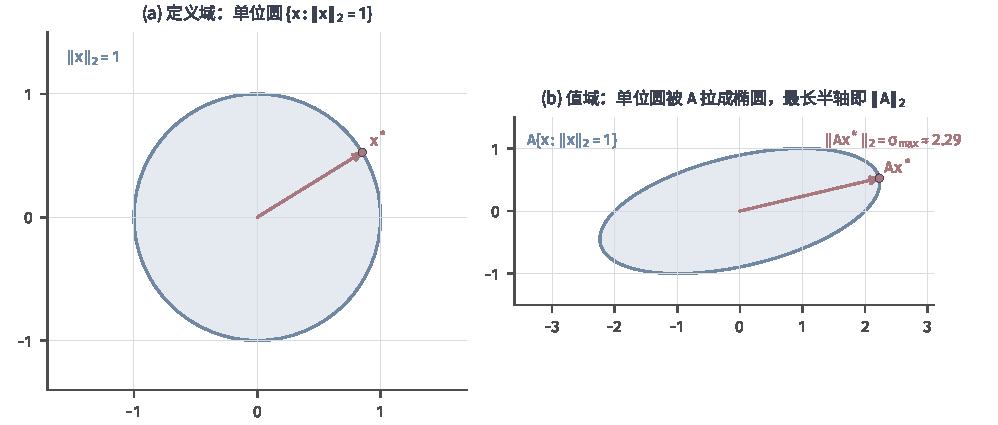
\includegraphics[width=169mm]{figures/00-shared/mathematical-preliminaries-upper/02-linear-spaces/matplotlib/ls-induced-norm-action/ls-induced-norm-action.pdf}
  \caption{诱导矩阵范数衡量最坏放大倍数。左：单位圆$\lVert\bm x\rVert_2=1$；中：同一线性作用$\bm A$把单位圆映成椭圆；右：椭圆上最长的轴给出$\lVert\bm A\rVert_2=\max_{\lVert\bm x\rVert_2=1}\lVert\bm A\bm x\rVert_2$，箭头指示最大放大方向。数值由$\bm A$的教学构造直接得到，是解析例。}
  \label{fig:ls-induced-norm-action}
\end{figure*}


\subsubsection{矩阵范数的性质}

\paragraph{列和与行和公式}
\[
 \begin{gathered}
 \lVert\bm A\rVert_1=\max_j\sum_i|a_{i,j}|,\\
 \lVert\bm A\rVert_\infty=\max_i\sum_j|a_{i,j}|.
 \end{gathered}
\]
第一式按列算：
\[
 \lVert\bm A\bm x\rVert_1=\Bigl\lVert\sum_jx_j\bm A_{:,j}\Bigr\rVert_1\leq\sum_j|x_j|\,\lVert\bm A_{:,j}\rVert_1\leq\Bigl(\max_j\lVert\bm A_{:,j}\rVert_1\Bigr)\lVert\bm x\rVert_1,
\]
而取$\bm x$为最大绝对列和所在列对应的标准坐标向量时等号成立。第二式按行算：对每个$i$，
\[
 |(\bm A\bm x)_i|\leq\sum_j|a_{i,j}|\,|x_j|\leq\Bigl(\sum_j|a_{i,j}|\Bigr)\lVert\bm x\rVert_\infty,
\]
对$i$取最大值即得上界；取输入各坐标为最大绝对行和那一行元素的符号（元素为零处取$1$），等号成立。

\paragraph{谱范数不超过Frobenius范数}
\[
 \begin{gathered}
 \lVert\bm A\bm x\rVert_2\leq\lVert\bm A\rVert_{\mathrm F}\lVert\bm x\rVert_2,\\
 \lVert\bm A\rVert_2\leq\lVert\bm A\rVert_{\mathrm F}.
 \end{gathered}
\]
对每行用$p=q=2$的Hölder不等式，$(\bm A\bm x)_i^2=(\bm A_{i,:}\bm x)^2\leq\lVert\bm A_{i,:}\rVert_2^2\lVert\bm x\rVert_2^2$；对$i$求和，右侧的$\sum_i\lVert\bm A_{i,:}\rVert_2^2$正是$\lVert\bm A\rVert_{\mathrm F}^2$，得到第一式。第一式说明每个比值$\lVert\bm A\bm x\rVert_2/\lVert\bm x\rVert_2$都不超过$\lVert\bm A\rVert_{\mathrm F}$，所以谱范数有限，并得到第二式。

对一般的输入、输出范数，由定理~\ref{thm:ls-norm-equivalence}，存在常数$c_1,c_2>0$，使
\[
 \begin{gathered}
 \lVert\bm y\rVert_\beta\leq c_1\lVert\bm y\rVert_2,\\
 \lVert\bm x\rVert_2\leq c_2\lVert\bm x\rVert_\alpha.
 \end{gathered}
\]
结合刚证明的Frobenius界，得到
\[
 \lVert\bm A\bm x\rVert_\beta
 \leq c_1c_2\lVert\bm A\rVert_{\mathrm F}\lVert\bm x\rVert_\alpha.
\]
所以定义中的上确界有限。

诱导范数满足范数的四条要求：非负性与齐次性由定义直接得到；若$\lVert\bm A\rVert_{\alpha\to\beta}=0$，则每个$\bm A\bm e_j=\bm0$，即$\bm A=\bm0$；三角不等式来自$\lVert(\bm A+\bm B)\bm x\rVert_\beta\leq\lVert\bm A\bm x\rVert_\beta+\lVert\bm B\bm x\rVert_\beta$，两边除以$\lVert\bm x\rVert_\alpha$再取上确界即得。

上确界还在某个方向达到。由齐次性，只需在输入范数单位球面$\{\bm x:\lVert\bm x\rVert_\alpha=1\}$上取上确界。上述下界保证该球面在欧氏坐标中有界，而范数的连续性保证坐标收敛的单位向量列，其极限仍在球面上。取输出范数趋于上确界的单位向量列，逐坐标抽取收敛子列；矩阵乘法和输出范数在坐标下连续，因而子列极限达到上确界。于是定义中的上确界可以写成最大值。

\paragraph{次乘性}
中间范数匹配时，
\[
 \lVert\bm A\bm B\rVert_{\alpha\to\gamma}
 \leq\lVert\bm A\rVert_{\beta\to\gamma}
 \lVert\bm B\rVert_{\alpha\to\beta}.
\]
连续应用两次诱导范数的界：
\[
 \lVert\bm A\bm B\bm x\rVert_\gamma\leq\lVert\bm A\rVert_{\beta\to\gamma}\lVert\bm B\bm x\rVert_\beta\leq\lVert\bm A\rVert_{\beta\to\gamma}\lVert\bm B\rVert_{\alpha\to\beta}\lVert\bm x\rVert_\alpha.
\]
两边除以$\lVert\bm x\rVert_\alpha$再取上确界即得。特别地，反复使用可得$\lVert\bm A^k\rVert_p\leq\lVert\bm A\rVert_p^k$。

\paragraph{Frobenius范数与谱范数的混合界}
\begin{equation}
\begin{gathered}
\lVert\bm A\bm B\rVert_{\mathrm F}
 \leq\lVert\bm A\rVert_2\lVert\bm B\rVert_{\mathrm F}\\
\lVert\bm A\bm B\rVert_{\mathrm F}
 \leq\lVert\bm A\rVert_{\mathrm F}\lVert\bm B\rVert_2.
\end{gathered}
\label{eq:matrix-analysis-mixed-submultiplicativity}
\end{equation}
第一式按列算：
\[
 \lVert\bm A\bm B\rVert_{\mathrm F}^2=\sum_j\lVert\bm A\bm B_{:,j}\rVert_2^2\leq\lVert\bm A\rVert_2^2\sum_j\lVert\bm B_{:,j}\rVert_2^2=\lVert\bm A\rVert_2^2\lVert\bm B\rVert_{\mathrm F}^2.
\]
第二式对转置应用第一式：$\lVert\bm A\bm B\rVert_{\mathrm F}=\lVert\bm B^\top\bm A^\top\rVert_{\mathrm F}\leq\lVert\bm B^\top\rVert_2\lVert\bm A^\top\rVert_{\mathrm F}$，其中转置不改变Frobenius范数，还需要说明$\lVert\bm B^\top\rVert_2=\lVert\bm B\rVert_2$。对固定的$\bm x$，由$p=q=2$的Hölder不等式，$\lVert\bm y\rVert_2=1$时$|\bm y^\top\bm B\bm x|\leq\lVert\bm B\bm x\rVert_2$，而$\bm B\bm x\neq\bm0$时取$\bm y=\bm B\bm x/\lVert\bm B\bm x\rVert_2$即取等号，所以
\[
 \lVert\bm B\rVert_2=\sup_{\lVert\bm x\rVert_2=\lVert\bm y\rVert_2=1}|\bm y^\top\bm B\bm x|.
\]
由于$\bm y^\top\bm B\bm x=\bm x^\top\bm B^\top\bm y$，交换$\bm x,\bm y$的角色，同一个上确界也等于$\lVert\bm B^\top\rVert_2$。结合$\lVert\bm A\rVert_2\leq\lVert\bm A\rVert_{\mathrm F}$，Frobenius范数也满足次乘性：$\lVert\bm A\bm B\rVert_{\mathrm F}\leq\lVert\bm A\rVert_{\mathrm F}\lVert\bm B\rVert_{\mathrm F}$。

\subsection{对偶范数}
\label{sec:ls-dual-norms}

上一章建立了线性泛函；这里已规定向量的大小，便可以进一步问一个读取规则有多“大”。先考虑$V=\mathbb R^d$，并取定该空间上的一种范数。这正是误差分析中的常见问题：误差$\bm r$只知道落在某个范数球内时，一次加权读取$\bm z^\top\bm r$最多变化多少？下面的量就是这个最大值。
\begin{definition}[对偶范数]
\label{def:linear-algebra-dual-norm}
给定$\mathbb R^d$上的范数，相对于标准坐标配对的\term{对偶范数}（dual norm）为
\begin{equation}
 \lVert\bm z\rVert_*=\sup_{\lVert\bm r\rVert\leq1}|\bm z^\top\bm r|.
 \label{eq:linear-algebra-dual-norm-definition}
\end{equation}
\end{definition}
对任意范数，这个上确界有限并可以取到（第~\ref{sec:ls-error-scale-comparison}节）；对$\ell_p$范数，下面还将直接构造取到它的$\bm r$。它满足范数的四条要求，因而是对偶空间上的范数。非负性显然。$\bm z\neq\bm0$时，取$\bm z$的某个非零坐标$z_j$，$\bm r=\bm e_j/\lVert\bm e_j\rVert$给出$|\bm z^\top\bm r|=|z_j|/\lVert\bm e_j\rVert>0$。对每个$\bm r$都有$|(\bm z+\bm w)^\top\bm r|\leq|\bm z^\top\bm r|+|\bm w^\top\bm r|$，取上确界即得三角不等式；齐次性由$|(c\bm z)^\top\bm r|=|c|\,|\bm z^\top\bm r|$得到。图~\ref{fig:ls-dual-norm-unit-ball}把这个最大值画成支撑线最后接触单位球的位置。

\begin{figure}[!htb]
  \centering
  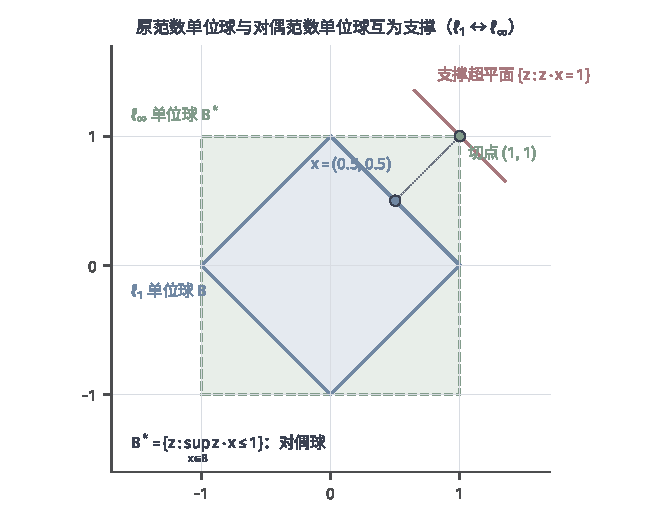
\includegraphics[width=112mm]{figures/00-shared/mathematical-preliminaries-upper/02-linear-spaces/matplotlib/ls-dual-norm-unit-ball/ls-dual-norm-unit-ball.pdf}
  \caption{对偶范数的几何：在原范数单位球$\lVert\bm r\rVert\leq1$上求线性读取$\bm z^\top\bm r$的最大值。左：原单位球（灰色）与读取方向$\bm z$；右：支撑直线最后接触单位球处给出$\lVert\bm z\rVert_*=\max_{\lVert\bm r\rVert\leq1}|\bm z^\top\bm r|$。对偶单位球（虚线）与原单位球互为极体，为解析教学例。}
  \label{fig:ls-dual-norm-unit-ball}
\end{figure}

对$\ell_p$范数，
\begin{equation}
\begin{gathered}
(\lVert\cdot\rVert_p)_*=\lVert\cdot\rVert_q\\
\frac1p+\frac1q=1,
\end{gathered}
\label{eq:linear-algebra-lp-duality}
\end{equation}
并且由齐次性，对$\rho\geq0$有
\begin{equation}
 \max_{\lVert\bm r\rVert_p\leq\rho}|\bm z^\top\bm r|
 =\rho\lVert\bm z\rVert_q.
 \label{eq:linear-algebra-linear-perturbation-duality}
\end{equation}
本节的Hölder不等式（定理~\ref{thm:linear-algebra-holder}）给出$\ell_p$单位球上的上界$\lVert\bm z\rVert_q$。这个上界可以达到：$1<p<\infty$且$\bm z\neq\bm0$时取$r_j=|z_j|^{q-1}\operatorname{sgn}(z_j)/\lVert\bm z\rVert_q^{q-1}$；$\bm z=\bm0$时上界为零，任取可行输入即可。$p=1$时把单位预算全部放在$|z_j|$最大的坐标上；$p=\infty$时逐坐标取$r_j=\operatorname{sgn}(z_j)$。下面固定一个读取，比较三种误差预算。
\begin{example}[同一读取在三种误差预算下的最大变化]
\label{ex:ls-dual-norm-three-budgets}
给定：读取方向$\bm z=(2,-1)^\top$，即读取$\bm z^\top\bm r=2r_1-r_2$。

计算：在$\ell_1$单位球上，把单位预算全部放在$|z_j|$最大的第一个坐标，$\bm r=(1,0)^\top$给出最大值$\lVert\bm z\rVert_\infty=2$。在$\ell_2$单位球上，取$\bm r=\bm z/\lVert\bm z\rVert_2=(2,-1)^\top/\sqrt5$，最大值为$\lVert\bm z\rVert_2=\sqrt5$。在$\ell_\infty$单位球上，逐坐标取$r_j=\operatorname{sgn}(z_j)$，$\bm r=(1,-1)^\top$给出最大值$\lVert\bm z\rVert_1=3$。若误差预算为$|r_j|\leq0.01$，在式~\eqref{eq:linear-algebra-linear-perturbation-duality}中取$p=\infty$、$\rho=0.01$，最大变化为$0.01\cdot(2+1)=0.03$，由$\bm r=(0.01,-0.01)^\top$达到。

结论：同一次读取在$\ell_1$、$\ell_2$、$\ell_\infty$单位球上的最大值依次为$2$、$\sqrt5$、$3$；改变误差预算的形状，最坏方向和最大变化都随之改变。
\end{example}
图~\ref{fig:linear-algebra-dual-unit-balls}画出这三种情形下的最坏方向。
\begin{figure*}[htbp]
  \centering
  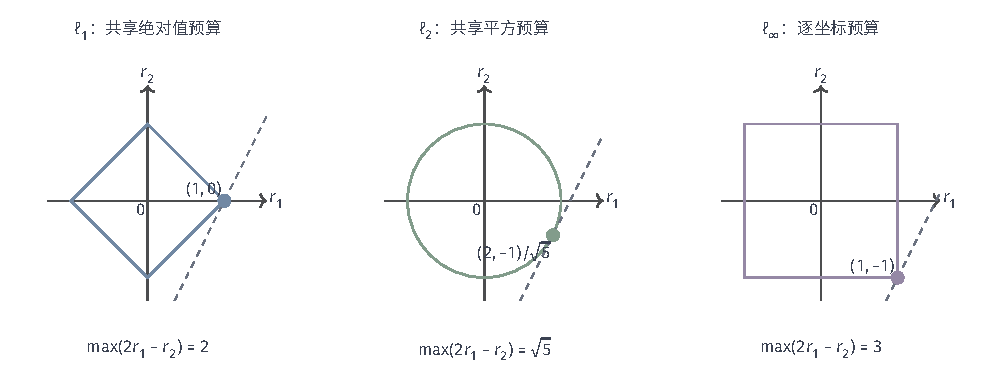
\includegraphics[width=168.998mm]{figures/00-shared/mathematical-preliminaries-upper/02-linear-spaces/tikz/linear-algebra-dual-unit-balls/figure.pdf}
  \caption{同一线性读取$2r_1-r_2$在$\ell_1$、$\ell_2$、$\ell_\infty$单位球上的最大值依次为$2$、$\sqrt5$、$3$。虚线为最后接触可行集的支撑直线，点为最大化方向。三图坐标尺度相同，均为解析教学例；改变允许误差的形状会改变误差常数。}
  \label{fig:linear-algebra-dual-unit-balls}
\end{figure*}

误差预算按$\ell_\infty$给出时，读取方向要按$\ell_1$计量；预算按$\ell_2$给出时，读取方向仍按$\ell_2$计量。所以讨论“输入误差最多引起多大输出误差”时，必须先说清误差用哪种范数度量。

\subsection{商范数}
\label{sec:ls-quotient-norms}

有限维子空间的闭性还可以用来为商空间定义范数。第~\ref{sec:ls-quotient-spaces}节的商空间$V/U$把相差$U$中向量的点看成同一个类$\bm x+U$，那里只建立了线性结构。同一类中各点到$U$的距离相同：若$\bm x'=\bm x+\bm u_0$，$\bm u_0\in U$，则$\bm u$遍历$U$时$\bm u-\bm u_0$也遍历$U$，所以$d(\bm x',U)=d(\bm x,U)$。因此可以把这个距离当作类的大小，称为商范数
\[
 \lVert\bm x+U\rVert_{V/U}=d(\bm x,U)=\inf_{\bm u\in U}\lVert\bm x-\bm u\rVert .
\]
它满足范数的三条要求。三角不等式：对任意$\bm u,\bm u'\in U$，$d(\bm x+\bm y,U)\leq\lVert(\bm x-\bm u)+(\bm y-\bm u')\rVert\leq\lVert\bm x-\bm u\rVert+\lVert\bm y-\bm u'\rVert$，再对$\bm u,\bm u'$分别取下确界。齐次性：$c\neq0$时$cU=U$，所以$d(c\bm x,U)=|c|\,d(\bm x,U)$；$c=0$时两边都为零。正定性要求$d(\bm x,U)=0$只在$\bm x+U=U$即$\bm x\in U$时发生，这正是上面的闭性结论。

\paragraph{一般范数下的最近点}
距离$d(\bm y,U)$定义为下确界，它总能取到吗？由$d(\bm y,U)\leq\lVert\bm y-\bm0\rVert=\lVert\bm y\rVert$，而$\lVert\bm u\rVert>2\lVert\bm y\rVert$时$\lVert\bm y-\bm u\rVert\geq\lVert\bm u\rVert-\lVert\bm y\rVert>\lVert\bm y\rVert$，所以只需在$K=\{\bm u\in U:\lVert\bm u\rVert\leq2\lVert\bm y\rVert\}$上找最小值。由子空间闭性，$K$是闭有界集，按“收敛与连续性”一段的最值论证，连续函数$\bm u\mapsto\lVert\bm y-\bm u\rVert$在其上取到最小值，所以最近点存在。

唯一性却可能失败。
\begin{example}[反例：$\ell_\infty$范数下最近点不唯一]
\label{ex:ls-linf-nonunique-nearest}
给定：$\mathbb R^2$取$\ell_\infty$范数，子空间$U=\operatorname{span}\{(1,0)^\top\}$，点$\bm y=(0,1)^\top$。

计算：$U$中的点写成$(t,0)^\top$，
\[
 \lVert\bm y-(t,0)^\top\rVert_\infty=\max\{|t|,1\}\geq1,
\]
等号当且仅当$|t|\leq1$时成立。

结论：$d(\bm y,U)=1$，所有满足$|t|\leq1$的点$(t,0)^\top$都是最近点，最近点不唯一。
\end{example}
内积诱导的范数下最近点唯一，并由正规方程算出（第~\ref{sec:ls-subspace-nearest-points}节）。
